\documentclass[12pt]{article}
\usepackage{amsmath,amssymb,amsfonts}
\usepackage{algorithmic}
\usepackage{graphicx}
\usepackage{float}
\graphicspath{ {./imgs/} }
\usepackage{textcomp}
\usepackage{xcolor}
\usepackage[margin=1in]{geometry}
\usepackage[portuguese]{babel}
\usepackage[style=ieee]{biblatex}
\addbibresource{~/.bibli.bib}
\addbibresource{bibli.bib}

\title{Alterando Binários ELF Manualmente\\ }
\date{15 de abril de 2020}

\author{
Mario Moura \\
Belém, Brasil \\
mario@mariomoura.com}
%\and
%\IEEEauthorblockN{2\textsuperscript{nd} Given Name Surname}
%\IEEEauthorblockA{\textit{dept. name of organization (of Aff.)} \\
%\textit{name of organization (of Aff.)}\\
%City, Country \\
%email address or ORCID}

\begin{document}


\maketitle

Cá estava eu programando com o nasm, tentando (apenas tentando mesmo) reproduzir os wrappers de systemcall que existem na glibc, quando me deparei com o tamanho de um bináriozinho em assembly que só retorna um valor, um "hello world" no nasm, ali no canto do diretório. O binário tinha 4.2K, nada realmente muito pesado, mas para um programa que não utiliza nenhuma biblioteca e só retorna um valor me pareceu muito estranho.

Código do programa:
\begin{verbatim}
BITS 32
global _start
_start:
    mov eax, 1
    mov ebx, 10
    int 0x80
\end{verbatim}
Para compilar e testar:

\begin{verbatim}
[mario@zrmt rivendell]$ nasm -f elf32 \
elrond.asm
[mario@zrmt rivendell]$ ld -m elf_i386 \
-s  elrond.o -o elrond
[mario@zrmt rivendell]$ ./elrond
[mario@zrmt rivendell]$ echo $?
10
\end{verbatim}
Aqui vai o hexdump do binário:

\begin{verbatim}
[mario@zrmt rivendell]$ hexdump -C elrond
00000000  7f 45 4c 46 01 01 01 00  00 00 00 00 00 00 00 00  |.ELF............|
00000010  02 00 03 00 01 00 00 00  00 90 04 08 34 00 00 00  |............4...|
00000020  20 10 00 00 00 00 00 00  34 00 20 00 02 00 28 00  | .......4. ...(.|
00000030  03 00 02 00 01 00 00 00  00 00 00 00 00 80 04 08  |................|
00000040  00 80 04 08 74 00 00 00  74 00 00 00 04 00 00 00  |....t...t.......|
00000050  00 10 00 00 01 00 00 00  00 10 00 00 00 90 04 08  |................|
00000060  00 90 04 08 0c 00 00 00  0c 00 00 00 05 00 00 00  |................|
00000070  00 10 00 00 00 00 00 00  00 00 00 00 00 00 00 00  |................|
00000080  00 00 00 00 00 00 00 00  00 00 00 00 00 00 00 00  |................|
*
00001000  b8 01 00 00 00 bb 2a 00  00 00 cd 80 00 2e 73 68  |......*.......sh|
00001010  73 74 72 74 61 62 00 2e  74 65 78 74 00 00 00 00  |strtab..text....|
00001020  00 00 00 00 00 00 00 00  00 00 00 00 00 00 00 00  |................|
*
00001040  00 00 00 00 00 00 00 00  0b 00 00 00 01 00 00 00  |................|
00001050  06 00 00 00 00 90 04 08  00 10 00 00 0c 00 00 00  |................|
00001060  00 00 00 00 00 00 00 00  10 00 00 00 00 00 00 00  |................|
00001070  01 00 00 00 03 00 00 00  00 00 00 00 00 00 00 00  |................|
00001080  0c 10 00 00 11 00 00 00  00 00 00 00 00 00 00 00  |................|
00001090  01 00 00 00 00 00 00 00                           |........|
00001098
\end{verbatim}
Da pra perceber que de \textbf{0x72} à \textbf{0xfff} todos os bytes são 0. Humm... suspeito. Não sou especialista e posso estar terrívelmente errado, mas não lembro dessa quantidade de zeros no manual do formato ELF. Se abrirmos o binário com o readelf veremos o seguinte:
\begin{verbatim}
[mario@zrmt rivendell]$ readelf elrond -h
ELF Header:
  Magic:   7f 45 4c 46 01 01 01 00 00 00 00 00 00 00 00 00
  Class:                             ELF32
  Data:                              2's complement, little endian
  Version:                           1 (current)
  OS/ABI:                            UNIX - System V
  ABI Version:                       0
  Type:                              EXEC (Executable file)
  Machine:                           Intel 80386
  Version:                           0x1
  Entry point address:               0x8049000
  Start of program headers:          52 (bytes into file)
  Start of section headers:          4128 (bytes into file)
  Flags:                             0x0
  Size of this header:               52 (bytes)
  Size of program headers:           32 (bytes)
  Number of program headers:         2
  Size of section headers:           40 (bytes)
  Number of section headers:         3
  Section header string table index: 2
\end{verbatim}

 Três \emph{Section Headers}, dois \textbf{Program Headers} e mais um bando de coisa. Como não precisamos das seções para executar o programa irei ignorá-las por agora. Não precisamos das seções para executar o programa devido ao fato de que elas são feitas para auxiliar o \emph{linker} no momento de construção do binário. Como o binário já está construído e nenhuma das seções representa objetos dinâmicos, elas podem ser ignoradas.

Então vamos diminuir esse programa aí. Primeiramente, devemos descobrir o endereço base do programa, para isto, basta pegar o \emph{entrypoint} (\textbf{0x8049000}) e diminuir o \emph{offset} do \textbf{Program Header} que tem a \emph{flag} de executável (que vai conter o devido código do programa). Lembrando que o \emph{entrypoint} é composto pelo endereço base do programa (para ser mapeado em memória) + “endereço” (no arquivo) do primeiro byte que corresponde ao código executável. O que vamos fazer aqui é achar esse primeiro byte, que pode ser encontrado no \textbf{Program Header}, onde se tem a flag de executável que recebe o nome de \textbf{p\_offset}. Vejamos o \textbf{readelf -l:}



\begin{verbatim}
[mario@zrmt rivendell]$ readelf -l elrond

Elf file type is EXEC (Executable file)
Entry point 0x8049000
There are 2 program headers, starting at offset 52

Program Headers:
  Type           Offset   VirtAddr   PhysAddr   FileSiz MemSiz  Flg Align
  LOAD           0x000000 0x08048000 0x08048000 0x00074 0x00074 R   0x1000
  LOAD           0x001000 0x08049000 0x08049000 0x0000c 0x0000c R E 0x1000

 Section to Segment mapping:
  Segment Sections...
   00
   01     .text
\end{verbatim}

 Para ajudar: de acordo com o manual o campo \textbf{p\_offset} é “O offset do início do arquivo onde o primeiro byte do segmento se encontra”. Como estamos lidando com um segmento executável esse primeiro byte vai ser o início do nosso código.

Então dá para ver que o segundo \textbf{Program Header} (que possui a \emph{flag} de executável) tem \emph{offset} \textbf{0x001000}! Então o endereço base é \textbf{0x08048000} (\textbf{0x08049000} - \textbf{0x00001000}) ! Já que temos o endereço base podemos excluir os zeros (caso contrário o programa ficaria quebrado e não iríamos conseguir analisá-lo com o readelf), alto lá! Apenas os inúteis! Mas quais são os inúteis ? Todos os que os \textbf{Program Headers} apontam, pois esses serão os  bytes do programa mapeados em memória, então vamos deixar eles lá. Vou usar o hyx como editor hexa, mas o hte também funciona.

Após excluirmos todos os zeros entre \textbf{0x74} e \textbf{0x1000}:


\begin{verbatim}
[mario@zrmt rivendell]$ hyx elrond
0000> 7f 45 4c 46 01 01 01 00 00 00 00 00 00 00 00 00 |.ELF............|
0010: 02 00 03 00 01 00 00 00 00 90 04 08 34 00 00 00 |............4...|
0020: 20 10 00 00 00 00 00 00 34 00 20 00 02 00 28 00 | .......4. ...(.|
0030: 03 00 02 00 01 00 00 00 00 00 00 00 00 80 04 08 |................|
0040: 00 80 04 08 74 00 00 00 74 00 00 00 04 00 00 00 |....t...t.......|
0050: 00 10 00 00 01 00 00 00 00 10 00 00 00 90 04 08 |................|
0060: 00 90 04 08 0c 00 00 00 0c 00 00 00 05 00 00 00 |................|
0070: 00 10 00 00 00 b8 01 00 00 00 bb 2a 00 00 00 cd |...........*....|
0080: 80 00 2e 73 68 73 74 72 74 61 62 00 2e 74 65 78 |...shstrtab..tex|
0090: 74 00 00 00 00 00 00 00 00 00 00 00 00 00 00 00 |t...............|
00a0: 00 00 00 00 00 00 00 00 00 00 00 00 00 00 00 00 |................|
00b0: 00 00 00 00 00 00 00 00 00 00 00 00 00 0b 00 00 |................|
00c0: 00 01 00 00 00 06 00 00 00 00 90 04 08 00 10 00 |................|
00d0: 00 0c 00 00 00 00 00 00 00 00 00 00 00 10 00 00 |................|
00e0: 00 00 00 00 00 01 00 00 00 03 00 00 00 00 00 00 |................|
00f0: 00 00 00 00 00 0c 10 00 00 11 00 00 00 00 00 00 |................|
0100: 00 00 00 00 00 01 00 00 00 00 00 00 00          |.............|
\end{verbatim}
Ahh muito mais enxuto! Porém o bicho tá todo quebrado. Se executarmos:

\begin{verbatim}
[mario@zrmt rivendell]$ ./elrond

Bus error (core dumped)
\end{verbatim}
 Um ``Bus error'' não é nada mais que uma tentativa de \emph{read} ou \emph{write} em um espaço de memória desalinhado. Como citado no manual os mapeamentos tem que ser alinhados com as páginas de memória, ou seja, 4KB.

Vamos consertá-lo! Vamos ter que consertar: o \emph{entrypoint} e o mapeamento do segundo \textbf{Program Header}, ou seja, seu endereço virtual, físico e seu \emph{offset}. Como estamos alterando as posições dos segmentos (isto é, o nome oficial para o que um \textbf{Program Header} mapeia)  teremos que alterar seu mapeamento no arquivo junto com o \emph{entrypoint} (que aponta para o primeiro byte de um segmento executável). Na verdade, o endereço físico pode ser ignorado, o manual cita que os “System V” ignoram endereços físicos de aplicações, mas iremos adicioná-los em prol da completude.

Revisando... o \emph{entrypoint} vai ser o \textbf{endereço base} mais o \emph{offset} do segundo \textbf{Program Header}, e esse offset vai ser \textbf{0x75} (lembre-se que era \textbf{0x1000}, mas com a retirada dos zeros entre \textbf{0x74} e \textbf{0x1000} efetivamente reduzimos o \emph{entrypoint} em \textbf{0xFFF} - \textbf{0x74} = \textbf{0xF8B},  logo, o \emph{entrypoint} vai ser \textbf{0x1000} - \textbf{0xF8B} = \textbf{0x75}) então nosso \emph{entrypoint} vai ser \textbf{0x08048075}. Esse também vai ser o \textbf{endereço virtual} e o \textbf{endereço físico} do header.

Então troquemos:
\begin{itemize}
	\item O entrypoint no Header ELF por 0x08048075
    \item O offset do section header por 0x00000075
    \item Os endereços virtuais e físicos do segundo Program Header por 0x08048075
\end{itemize}
 Agora mais do que nunca teremos que ter atenção. Saque seu editor de hexa preferido e lembre-se que estamos lidando com little endian. Vou usar o hyx, que é um editor hexa um pouco parecido com o vi:


\begin{figure}[H]
	\centering
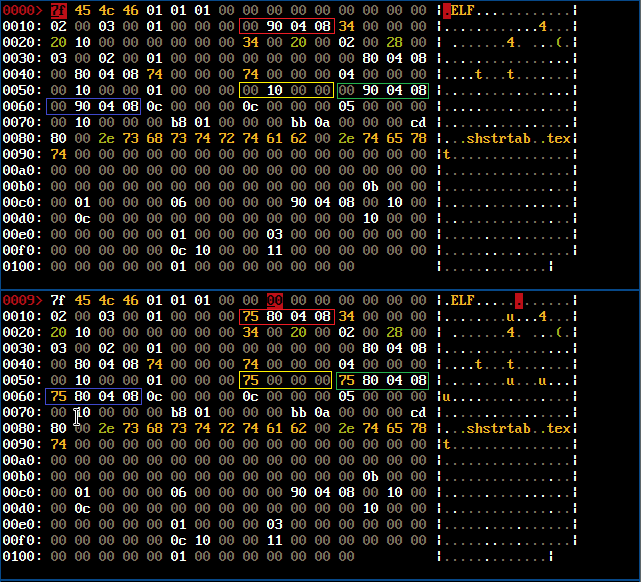
\includegraphics[scale = 1.00]{img1.png}
	\centering
\end{figure}

No terminal de cima temos o arquivo original sem os zeros, já no de baixo temos o arquivo já alterado.

Para ajudar:
\begin{itemize}
	\item Vermelho: Entrypoint
    \item Amarelo: Offset do Header
    \item Verde: Endereço Virtual do Header
    \item Azul: Endereço Físico do Header
\end{itemize}
Agora se executarmos:
\begin{verbatim}
[mario@zrmt rivendell]$ ./elrond
[mario@zrmt rivendell]$ echo $?
10
\end{verbatim}
Como disse lá em cima, não alterei as seções e \textbf{nesse caso} (binário já linkado e sem bibliotecas dinâmicas) elas não são importantes. Tente ler elas pra ver o que acontece.

No fim passamos de 4.2k para ...

\begin{verbatim}
[mario@zrmt rivendell]$ ls -lh elrond
-rwxr-xr-x 1 mario mario 269 --- -- --:-- elrond
\end{verbatim}
269!

Achei que a galera poderia gostar dessa pequena aventura, acho bem interessante principalmente para aprender bem sobre o formato. Se gostarem tenho planos pra parte dois!


\end{document}
